%
% LaTeX template for prepartion of submissions to PLDI'15
%
% Requires temporary version of sigplanconf style file provided on
% PLDI'15 web site.
%
\documentclass[pldi]{sigplanconf-pldi15}

%
% the following standard packages may be helpful, but are not required
%
\usepackage{SIunits}            % typset units correctly
\usepackage{courier}            % standard fixed width font
\usepackage[scaled]{helvet} % see www.ctan.org/get/macros/latex/required/psnfss/psnfss2e.pdf
\usepackage{url}                  % format URLs
\usepackage{listings}          % format code
\usepackage{enumitem}      % adjust spacing in enums
\usepackage[linesnumbered,ruled]{algorithm2e}
\usepackage{algpseudocode}
\usepackage{graphicx}
\usepackage[colorlinks=true,allcolors=blue,breaklinks,draft=false]{hyperref}   % hyperlinks, including DOIs and URLs in bibliography
% known bug: http://tex.stackexchange.com/questions/1522/pdfendlink-ended-up-in-different-nesting-level-than-pdfstartlink
\newcommand{\doi}[1]{doi:~\href{http://dx.doi.org/#1}{\Hurl{#1}}}   % print a hyperlinked DOI



\begin{document}

%
% any author declaration will be ignored  when using 'plid' option (for double blind review)
%

% TODO: Don't forget to run e.g. s/\\quicksand /\\quicksand~/
\newcommand\landslide{\textsc{Landslide}}
\newcommand\quicksand{\textsc{Quicksand}}
\newcommand\simics{\textsc{Simics}}
\newcommand{\sect}[1]{\S #1}
\newcommand\hilight[2]{\color{#1}#2\color{black}}
\definecolor{olivegreen}{RGB}{0,127,0}
\definecolor{brickred}{RGB}{192,0,0}

% TODO: Finalize these numbers.
\newcommand\numthrlibs{79}
\newcommand\numpintoses{79}
\newcommand\numstudence{158} % total pintoses plus p2s

\title{Stateless Model Checking with Data-Race Preemption Points}
\authorinfo{Ben Blum}{Carnegie Mellon University}{bblum@cs.cmu.edu}
\authorinfo{Garth Gibson}{Carnegie Mellon University}{garth@cs.cmu.edu}

\maketitle
\begin{abstract}
Stateless model checking is a promising technique for testing concurrent programs,
but is vulnerable to exponential explosion of the state space when the test input parameters are too large.
Several partial-order reduction techniques exist for mitigating this explosion,
but even after pruning equivalent interleavings, the state space size for a fixed set of preemption points is unpredictable and often intractable.
%
Data race detection, another concurrency testing approach, focuses on identifying suspicious memory access pairs during a single test execution.
It avoids concerns of intractable state space size, but suffers from a high rate of false positives.

We present an {\em Iterative Deepening} framework for stateless model checking,
which manages the exploration of many state spaces using different subsets of preemption points.
It uses state space estimation to prioritize jobs most likely to complete in a fixed CPU budget,
and it incorporates a data-race analysis to dynamically add new preemption points to verify each data race as buggy or benign.
%
Our evaluation shows this technique is
more effective than single-state-space model checking, both at finding more bugs and at completing more state spaces when no bug exists.

\end{abstract}

%%%%%%%%%%%%%%%%%%%%%%%%%%%%%%%%%%%%%%%%%%%%%%%%%%%%%%%%%%%%%%%%%%%%%%%%%%%%%%%%

\section{Introduction}

% blah blah trite opening sentence
%As parallelism becomes ever more important for achieving high performance in modern-day programs,
%so too do advanced concurrency testing techniques become important for verifying the correctness of those programs.
Concurrency bugs are notoriously hard to find and reproduce because they only appear in specific thread interleavings, which arise at random during normal program execution.
{\em Stateless model checking} \cite{verisoft} offers a method for finding such bugs,
or verifying their absence,
%by systematically executing a program along as many distinct interleavings as possible,
by forcing a program to execute each distinct interleaving,
capturing and controlling this nondeterminism using a finite state space.
Unfortunately, these state spaces explode exponentially in the size of the input program.
Reduction techniques such as Dynamic Partial Order Reduction \cite{dpor} and Maximal Causality Reduction \cite{mcr} expand the limits of feasible test completion,
and search ordering strategies such as Iterative Context Bounding \cite{chess-icb} allow bugs to be found sooner in a given exploration should they exist.

% Can I even make a claim this broad to begin with?
However, all stateless model checkers to date are bound by a fixed set of {\em preemption points}: code locations that define the granularity at which threads interleave.
% TODO: You repeat the following 1.5 sentence in the related work section; maybe you can eliminate this redundancy to save space?
For example, \textsc{CHESS} \cite{chess} preempts only on synchronization operations and library calls, which can miss lock-free shared memory races.
It provides an additional data-race analysis to report any violations of this model;
however, data-race analyses are prone to report false positives
%and benign races
which require annotations or imprecise heuristics to suppress \cite{racerx,tsan,datacollider}.
%
On the other hand, SPIN \cite{spin}
is able to preempt threads around any shared memory access. Such fine granularity would automatically check if each data race is a real bug, but makes full state space completion intractable for even modestly-sized tests.
%
Configuring a model checker is a tradeoff between schedule coverage and feasibility of completion.
This work shows how to avoid making that tradeoff decision in advance.

% TODO: ttuttle says this is too much of a jump -- that exactly what "subsets" means is not well defined (i.e, lock vs unlock, while NOT addressing the within/without_function problem)

We present \quicksand, a framework for {\em Iterative Deepening} of preemption points during stateless model checking.
Named after the analogous technique in chess AI \cite{iterative-deepening-chess-ai}, our approach likewise makes progressively deeper searches of the state space until a given CPU budget is exhausted.
Rather than attempting to search a single state space with every available preemption point enabled (e.g., preempting on every pthread API call),
\quicksand~tests many different state spaces corresponding to subsets of those points, managing a model checker instance to explore each one.
It estimates the size of each state space to decide when long-running instances should be suspended, and dynamically generates new state spaces based on data race analysis.
%In fact, if given enough time to fully test all discovered data-race preemption points,
%Iterative Deepening provides a full verification of all thread schedules that could arise from preempting anywhere.
In fact, Iterative Deepening is fully general:
we prove that if it completes all state spaces resulting from data-race preemption points,
that serves as a total verification of all possible thread interleavings of the given test program.

We evaluate \quicksand~by testing \numstudence~student thread libraries and kernels from the undergraduate OS classes at Carnegie Mellon, Berkeley, and the University of Chicago.
\quicksand~finds more bugs than the conventional stateless model checking approach given the same CPU budget,
% joshua wants me to say "conventional approachES" here
and furthermore, adding data-race preemption points quickly exposes bugs missed by even the ``maximal'' state space of the conventional approach.

This paper's contributions are as follows:
\begin{enumerate}
	\item Iterative Deepening, a new technique for combining data-race analysis with stateless model checking, and \quicksand, an open-source implementation of the technique;
	\item A proof of convergence, which shows that should it be possible in the given CPU budget,
		fully testing every discovered data-race preemption point is equivalent to testing all possible thread schedules;
	\item A new tactic for eliminating one class of false-positive data races,
		which cannot soundly be used in a single-pass analysis,
		but which we prove correct when used with Iterative Deepening;
		%, unsound in single-pass analysis but which we prove sound when used with Iterative Deepening;
	%\item Techniques for detecting and flattening cyclic state spaces resulting from ad-hoc while-loop synchronization % TODO: is there actually room for this in the paper?
	\item A large evaluation in which \quicksand~compares favorably to stand-alone data-race detection and stateless model checking approaches.
\end{enumerate}

The remainder of the paper is organized as follows.
\sect{\ref{sec:design}} discusses the background and design of Iterative Deepening, including our proof of convergence,
\sect{\ref{sec:implementation}} explains \quicksand's approach to implementing it, including our new false-positive data-race tactic,
\sect{\ref{sec:eval}} presents our evaluation,
\sect{\ref{sec:future}} discusses limitations and future work,
\sect{\ref{sec:related}} surveys the related work,
and \sect{\ref{sec:conclusion}} concludes.

\section{Definitions}

\subsection{System Model}

To reason about programs at the executable level, we will define them as a list of assembly-like instructions,
including certain concurrency primitives which we evaluate atomically, assuming the runtime provides correct implementations for them.
\begin{eqnarray*}
	\mathcal{P} &::=& [n, \mathcal{I}] \\
	\mathcal{I} &::=& v \leftarrow \mathsf{read}(a) \quad | \quad \mathsf{write}(a,v) \quad | \quad \mathsf{xchg}(a,v) \\
	&|& a \leftarrow \mathsf{malloc}(n) \quad | \quad \mathsf{free}(a) \\
	&|& \mathsf{mutex\_lock}(m) \quad | \quad \mathsf{mutex\_unlock}(m) \\
	&|& \mathsf{deschedule} \quad | \quad \mathsf{make\_runnable}(t) \\
	&|& t \leftarrow \mathsf{thread\_fork} \quad | \quad \mathsf{thread\_exit} \quad | \quad \mathsf{yield} \\
	&|& \textit{local}
\end{eqnarray*}

The execution state consists of any number of threads, each represented by a list of instructions to execute ($[\mathcal{I}]$),
a stack of variable maps for thread-local state ($v$),
and an indicator of whether the thread is runnable.
The state also includes a map of global memory, indexed by addresses denoted $a$,
and a set of mutex objects, denoted $m$. Thus:
\begin{eqnarray*}
	\mathcal{E} &::=& [\mathcal{T}] \times [a \rightarrow \mathsf{int}] \times [m \rightarrow \mathsf{bool}] \\
	\mathcal{T} &::=& \mathcal{P} \times [[v \rightarrow \mathsf{int}]] \times \mathsf{bool}
\end{eqnarray*}
For the sake of brevity, we will not explicitly define execution semantics, though they are straightforward:
To execute one step, arbitrarily choose one runnable thread, and evaluate the first element of its instruction list.
This gives rise to thread concurrency which can interleave at instruction granularity,
although it assumes a sequentially-consistent memory model. For a treatment of DPOR with relaxed memory, we refer the reader to \cite{tsopso}.

{\bf Memory.} $\mathsf{read}$, $\mathsf{write}$, and $\mathsf{xchg}$ access global or heap memory shared by all threads, indicated by some address $a$, and copying and/or modifying a thread-local variable $v$. % cmpxchg, xadd, etc omitted for brevity
$\mathsf{malloc}$ and $\mathsf{free}$ provide access to fresh memory accessible by all threads. % free is irrelevant to the system model in terms of expressive power

{\bf Threads.} $\mathsf{mutex\_lock}$ and
$\mathsf{mutex\_unlock}$ provide mutual exclusion:
a thread cannot evaluate $\mathsf{mutex\_lock}$ until that lock is released.
$\mathsf{deschedule}$ and $\mathsf{make\_runnable}$ allow threads to manipulate their own or another's runnability, respectively,
and $\mathsf{thread\_fork}$ and $\mathsf{thread\_exit}$ allow creation and destruction of new threads.
$\mathsf{thread\_fork}$ is defined in the Pebbles manner \cite{kspec};
we omit higher-level abstractions such as $\mathsf{create}$ or $\mathsf{join}$, which can be implemented using these primitives \cite{thrlib}.
$\mathsf{yield}$ has no effect under these execution semantics, but is included for the sake of synchronization API preemption points (see below).

{\bf Local state.}
$\textit{local}$ represents any thread-local instruction, such as modifying local variables, flow control, function definition/calling, assertions, and side effects.
For brevity, we omit a detailed list, although note that $\mathsf{call}$ would be implemented by modifying the instruction stream $[\mathcal{I}]$ and creating a new frame on the stack of local variables.

\begin{definition}[Blocked threads]
	A thread is blocked when either its runnable flag is false, or when its next instruction is a $\mathsf{mutex\_lock}$ on an unavailable mutex.
\end{definition}

Model checkers often also include heuristics to identify threads using open-coded $\mathsf{yield}$ loops to block,
but for the sake of our proofs, we assume such patterns are implemented more tastefully with a condition-variable-like primitive built upon $\mathsf{deschedule}$.

\begin{definition}[Interleaving]
	An interleaving is a sequence of execution steps, beginning with some initial program state and ending when all threads are blocked or have exited, and/or when a bug is observed.
\end{definition}

\subsection{Stateless model checking terms}

\begin{definition}[Preemption point (PP)]
	%A PP is a code location between two instructions at which we may force threads to switch.
	A PP is a predicate on the execution state which identifies a class of instruction pairs between which we may force threads to switch.
\end{definition}

In the main paper, we identified PPs by predicates on the instruction pointer and current thread ID. Hence, the ``same'' PP may occur multiple times during an execution; for example, {\tt mutex\_lock()} may be called from {\tt foo()} and later again from {\tt bar()}.
%For the sake of this proof, we separate such cases into multiple unique PPs: each PP is simply a label denoting the end of a single transition.
In our proofs, we will use the term ``PP'' to indicate specific instruction sites at which a PP predicate holds.

We also use ``synchronization API PPs'' to denote the class of
%statically-available
PPs which occur immediately {\em after} any of
$\mathsf{mutex\_lock}$,
$\mathsf{mutex\_unlock}$,
$\mathsf{deschedule}$,
$\mathsf{make\_runnable}$,
$\mathsf{thread\_fork}$,
$\mathsf{thread\_exit}$,
$\mathsf{yield}$.
Because no other instruction affects a thread's runnability, it is always possible to execute a program by switching the currently-executing thread only at synchronization API PPs.

All data-race PPs will occur immediately {\em before} a $\mathsf{read}$, $\mathsf{write}$, or $\mathsf{xchg}$.

\begin{definition}[Transition]
A sequence of execution steps from a program's evaluation between two preemption points (PPs).
\label{def:transition}

\end{definition}
We require the invariant that each transition's instructions are associated with exactly one thread. (That is, the set of PPs always includes all thread switches.)
The set of synchronization API PPs provides this invariant, and all other PP sets in these proofs will be supersets of those.
We also assume a trace of all memory accesses is available in the representation of transitions.

\begin{definition}[State space]
Given a set of PP predicates, a state space is
a set of interleavings representing all possible execution sequences which switch threads only on those PPs.
\end{definition}

\begin{definition}[Must-happen-before (MHB)]
%Given two transitions $A$ and $B$, we say $A$ MHB $B$ if $B$ cannot be reordered to occur before $A$.
Let $t_1$ and $t_2$ be two transitions of an interleaving, and $T1$ and $T2$ be the corresponding thread IDs,
and let $t_1$ occur before $t_2$.
Then $t_1$ MHB $t_2$ if
\begin{enumerate}
	\item $T2$ is blocked immediately preceding $t_1$ and not blocked immediately afterward,
		and there does not occur another $t_2'$ by $T2$ between $t_1$ and $t_2$; or
	\item there occurs some $t_3$ by thread $T3$ such that $t_1$ MHB $t_3$, $t_3$ MHB $t_2$, and $T3 \ne T2$; or
	\item $T1 = T2$.
\end{enumerate}
\end{definition}

Intuitively, MHB expresses the "cannot be reordered with" (or "enables") relation between transitions.
Two transitions $A$ and $B$ of different threads MHB if some synchronization event in $A$ causes $B$ to become runnable while it was previously blocked. Such synchronization events include {\tt thread\_create}, {\tt cond\_signal}, {\tt sem\_post}, but {\em not} {\tt mutex\_lock} or {\tt mutex\_unlock}.

Note how our {\em must}-happen-before relation differs from the conventional definition of happens-before (``observed to happen before'') \cite{lamport-clocks}.
Our use of MHB matches the ``limited happens-before'' used in \cite{hybriddatarace} and \cite{tsan};
the advantage of this over pure-happens-before detectors in producing fewer false negatives is well-argued in those prior works\footnote{
Because pure-HB data race detectors avoid false positives altogether, they would have no trouble avoiding our malloc-recycle false positives.
However, as prior work has shown, they miss many other bugs involving unprotected variables accessed alternately before and after mutex-protected critical sections.
%Indeed, because most concurrent malloc implementations are protected by a lock,
%our malloc-recycle false positives are indistinguishable from such false negatives under pure-HB.
}.
We illustrate the difference in Figure~\ref{fig:mhb}.

\begin{figure}[t]
	\small
\begin{tabular}{rll}
	& Thread 1 & Thread 2 \\
	1 & \texttt{\hilight{brickred}{my\_x->foo = ...;}} & \\
	2 & \texttt{\hilight{olivegreen}{mutex\_lock(...);}} &\\
	3 & \texttt{global\_x = my\_x;} & \\
	%4 & \texttt{\hilight{olivegreen}{yield();}} & \\
	4 & \texttt{\hilight{olivegreen}{mutex\_unlock(...);}} & \\
	5 & & \texttt{\hilight{olivegreen}{mutex\_lock(...);}} \\
	6 & & \texttt{my\_x = global\_x;} \\
	7 & & \texttt{\hilight{olivegreen}{mutex\_unlock(...);}} \\
	8 & & \texttt{if (my\_x != NULL)} \\
	9 & & \texttt{\hilight{brickred}{~~~~my\_x->foo = ...;}} \\
\end{tabular}
	\caption{Example program to illustrate the difference between {\em pure happens-before} and {\em must-happen-before}.
	Under pure happens-before (which does not identify false positives), lines 1 and 9 are not a data race candidate.
	Under MHB, they are; although after trying to reorder them, it will be classified as a false positive.}
	\label{fig:mhb}
\end{figure}

Note also that although transitions of the same thread are related by MHB,
MHB is transitive only when the latter two transitions are not by the same thread (condition 2).
While lock-protected critical sections can be reordered around each other (i.e., line 1 not MHB lines 8-9),
one cannot be reordered to be in the middle of the other (i.e, lines 3-4 MHB line 6).
%Hence, MHB is not necessarily transitive.
In the latter case, the MHB relation is established by the mutex's blocking mechanism used during contention.

In our main paper, we refer to this relation (in conjunction with a lock-set analysis) as Limited HB.

\begin{definition}[Shared memory conflict]
A pair of memory accesses between two threads to the same address where at least one of them is a write.
\end{definition}

% Outdated. See above.
%\begin{definition}[Interleaving]
%	An ordered list of transitions and preemption points between them.
%\end{definition}

\begin{definition}[Independent transitions]
Two transitions between different threads are independent if the intersection of their shared memory accesses contains no conflicts.
\end{definition}

\begin{definition}[Equivalent interleaving]
Two interleavings are equivalent if one can be transformed into the other by permuting only independent transitions.
\end{definition}

Intuitively, the behaviour of a program could change by reordering two transitions only if they contain a memory conflict.
All possible interleavings of a program can be partitioned into equivalence classes,
so only one interleaving from each equivalence class need be tested to ensure total schedule coverage \cite{mazurkiewicz}.

% Outdated. See above.
%\begin{definition}[State space]
%	A set of interleavings subject to the constraint that, given the preemption points used, all equivalence classes of possible interleavings are represented by at least one member.
%\end{definition}

\begin{definition}[Dynamic Partial Order Reduction (DPOR)]
	A state-space search algorithm for stateless model checkers;
	given a state space $\mathcal{S}$, it will test at least one interleaving from each equivalence class in $\mathcal{S}$.
	%guaranteed to reorder transitions of two threads
	%iff they are not independent and are not related by MHB \cite{dpor}.
	\label{def:dpor}
\end{definition}

Considering an interleaving $\mathcal{I}$ in $\mathcal{S}$, if two transitions $t_1$ and $t_2$ by different threads are not independent and not related by MHB, let $\mathcal{J}$ be the interleaving which reorders $t_1$ with $t_2$. DPOR is then guaranteed to test some interleaving in $\mathcal{S}$ equivalent to $\mathcal{J}$ \cite{dpor}.

Because equivalent interleavings produce identical execution states,
DPOR guarantees to expose all reachable execution states by testing its subset of interleavings.
We refer to this property as {\em the soundness of DPOR}.

%The soundness of DPOR guarantees that if a program behaviour can possibly be exposed by any thread interleaving around the given transitions/PPs,
%that interleaving will eventually be tested by reordering only such conflicting transitions.
%In other words, reordering memory-independent thread transitions cannot possibly affect program behaviour.

\subsection{Data race and other memory terms}

\begin{definition}[Data race]
A shared memory conflict where furthermore:
\begin{itemize}
	\item The intersection of both threads' locksets is empty (i.e., the threads do not hold the same lock during each access), and
	\item The threads' transitions are not related by MHB.
\end{itemize}
\end{definition}

The same as in the paper, we distinguish between data-race {\em candidates} (or {\em potential} data races) and data-race {\em bugs}.
For brevity, we now use ``data race'' to refer both to true races and to potential data-race candidates identified by MHB.
In this proof we are concerned solely with candidates, and whether they can be observed to race or are false positives.
It is up to the MC to decide whether true data races are benign or buggy.

\begin{definition}[False positive data race]
	An apparent data race that cannot be observed in the opposite order from what was actually executed.
\end{definition}

False positives are caused when some data dependency based on some other shared state, invisible to the data-race analysis,
changes some variable values when the threads are reordered, such that the memory addresses no longer collide.

\begin{definition}[Malloc-recycle data race]
	A data race where the address is contained in some heap-allocated memory, and between the two accesses, that memory was passed to free() and returned again by a subsequent malloc().
\end{definition}

Figures~\ref{fig:recycle} and \ref{fig:recycle-bug} show an example.
In the case of malloc-recycle false positives, the allocation heap is the ``other shared state'' mentioned in the previous definition, and malloc's return value is the variable value that changed.

Recent work \cite{sparc-ssm} has proposed hardware techniques for detecting many classes of stale heap pointer accesses, including the one shown in Figure \ref{fig:recycle-bug}.
This approach could be combined with stateless model checking in future work to identify such bugs immediately,
rather than requiring Iterative Deepening to explore new state spaces corresponding to the data race.
However, if the {\tt malloc} call were in thread 1 instead of thread 2, the bug would still be nondeterministic, requiring stateless model checking to expose.

\begin{definition}[Use after free]
	Any read or write to heap memory which was once allocated, but no longer is.
\end{definition}

These can immediately be identified as failures by a MC which tracks allocation state.
%Most commonly this refers to accesses to a region already freed, but for brevity we also include

\begin{figure}[t]
	\small
\begin{tabular}{rll}
	& \multicolumn{2}{c}{\texttt{struct x \{ int foo; int baz; \} *x;}} \\
	& \multicolumn{2}{c}{\texttt{struct y \{ int bar; \} *y;~~~~~~~~~~}} \\
	\\
	& Thread 1 & Thread 2 \\
	1 & \texttt{\hilight{brickred}{x1->foo = ...;}} & \\
	2 & \texttt{\hilight{olivegreen}{free}(x1);} \\
	3 & & \texttt{\hilight{commentblue}{// x's memory recycled}} \\
	4 & & \texttt{y~=~\hilight{olivegreen}{malloc}(sizeof *y);} \\
	5 & & \texttt{\hilight{commentblue}{// ...initialize...}}\\
	6 & & \texttt{publish(y);} \\
	7 & & \texttt{\hilight{brickred}{y->bar = ...;}} \\
\end{tabular}
\caption{False-positive malloc-recycle pattern. This is the common case for which we avoid creating new state spaces.}
\label{fig:recycle}
\end{figure}

\begin{figure}[t]
	\small
\begin{tabular}{rll}
	& Thread 1 & Thread 2 \\
	1 & \texttt{publish(x1);} & \\
	2 & & \texttt{x2 = get\_published\_x();} \\
	3 & \texttt{\hilight{brickred}{x1->foo = ...;}} & \\
	4 & \texttt{\hilight{olivegreen}{free}(x1);} \\
	5 & & \texttt{\hilight{commentblue}{// x's memory recycled}} \\
	6 & & \texttt{y~=~\hilight{olivegreen}{malloc}(sizeof *y);} \\
	7 & & \texttt{\hilight{brickred}{x2->foo = ...;}} \\
\end{tabular}
\caption{Adversarial program which fits the malloc-recycle pattern, but nevertheless contains a true race.}
\label{fig:recycle-bug}
\end{figure}

\begin{figure}[t]
	\small
\begin{tabular}{rll}
	& Thread 1 & Thread 2 \\
	1 & \texttt{publish(x1);} & \\
	2 & & \texttt{x2 = get\_published\_x();} \\
	3 & & \texttt{\hilight{commentblue}{// x not free, so malloc's}} \\
	4 & & \texttt{\hilight{commentblue}{// return value changes!}} \\
	5 & & \texttt{y~=~\hilight{olivegreen}{malloc}(sizeof *y);} \\
	6 & & \texttt{\hilight{brickred}{x2->foo = ...;}} \\
	7 & \texttt{\hilight{brickred}{x1->foo = ...;}} & \\
	8 & \texttt{\hilight{olivegreen}{free}(x1);} \\
\end{tabular}
\caption{Goal interleaving, which reorders the adversarial program's threads away from the pattern, while the data race remains.}
\label{fig:recycle-goal}
\end{figure}

%%%%%%%%%%%%%%%%%%%%%%%%%%%%%%%%%%%%%%%%%%%%%%%%%%%%%%%%%%%%%%%%%%%%%%%%%%%%%%%%

\section{Intuition}

In this section we provide (hopefully) intuitive summaries of both our proof goals.
%for readers not interested in double-checking the proofs' internal structure.

{\bf Intuition for Iterative Deepening convergence.}
In summary, we are proving that when Iterative Deepening finishes saturating the set of available data-race PPs,
that set represents every single code location where a preemption could possibly affect the program's behaviour,
and that completing the associated state spaces is as strong of a verification as testing all possible thread interleavings under any preemptions anywhere.
Some data-races may be hidden in control-flow paths which could only be executed after preempting on a different data-race,
but the technique's iterative nature will eventually find it.
On the other hand, relying on the soundness of DPOR, preempting on an instruction which is neither a data-race or sync API boundary cannot affect the program's behaviour,
so any PPs beyond the ones we consider are irrelevant.

{\bf Intuition for malloc-recycle soundness.}
In summary, we are proving that if a malloc-recycle-pattern data race is a true race, rather than a false positive,
then DPOR is guaranteed to ``reorder away the free and re-malloc''.
In other words, DPOR's exploration will eventually interleave threads in such a way that the malloc-recycle pattern will disappear,
while the access pair remains for the data-race detector to find, as shown in Figure~\ref{fig:recycle-goal}.
Hence, in the same state space where the malloc-recycle data race was found, if it's a true race, the same race will also appear without the recycle pattern.
So if that race hides a failure bug (assertion, segfault, etc.), Iterative Deepening will still be led to the necessary preemption point to find that bug.

\section{Evaluation}
\label{sec:eval}

Although \quicksand~presents Iterative Deepening and data-race PPs as interconnected techniques, they each could be employed alone as well. %in other model checkers.
For example, a single-state-space tool could use data-race PPs during immediately subsequent interleavings,
%essentially
changing the state space on the fly.
Likewise, a message-passing-only tool could use Iterative Deepening despite a concurrency model lacking data races, % being absent from its concurrency model.
to promote completing subset PP sets for large tests.
Hence, though many of our experiments compare \quicksand~to the state-of-the-art as a whole,
we also evaluated each technique individually.
Our evaluation answers the following questions:
\begin{enumerate}

	\item Does \quicksand~improve upon state-of-the-art MC?
		\begin{enumerate}
			\revision{\item} Do data-race PPs expose new bugs that couldn't be found with SSS-MC's fixed-PP-set approach?
				% Elaborate later:
				% Among those, how many were missed in a {\em completed} execution of the otherwise ``maximal'' state space?
			\revision{\item} Does Iterative Deepening find bugs faster
				%than SSS-MC
				in subset state spaces, even without data-race PPs?
			% Probably not... ICB is state of the art here.
			% In large tests, can Iterative Deepening provide partial verification by completing smaller state spaces
			\revision{
			\item Does Iterative Deepening provide more full verifications of bug-free programs more quickly?
			}
		\end{enumerate}
	\item Does MC improve the accuracy of data-race detection?
		\begin{enumerate}
			\item Do we avoid false positives compared to a single-execution data race analysis?
				% Explain later as:
				% How many data-race candidates were verified as benign
				% But to be fair, you have to count how many DRs are reported as "couldn't test these, check yourself" at the end.
				% Also Include:
				% How many false positives does the free-re-malloc technique suppress?
				% to do (done) If you have time, re-run all of the dr-only bug tests, with DR_FALSE_NEG enabled, and see how much fewer bugs get found (how many bugs get pushed past the time limit?)
				% Answer: Just 1. (for p2s at least; as of time of writing, pintos dr-falsenegs not run yet)
			\item Do we find data-race bugs that would be false-negatives during a single-execution analysis?%Do we avoid false negatives compared to single-pass?
		\end{enumerate}
\end{enumerate}

%%%%%%%%%%%%%%%%%%%%%%%%%%%%%%%%%%%%%%%%%%%%%%%%%%%%%%%%%%%%%%%%%%%%%%%%%%%%%%%%

\subsection{Test Suite}
\label{sec:testsuite}
Our test suite consists of \numthrlibs~``P2'' student thread libraries, from Carnegie Mellon's 15-410 operating systems class,
and \numpintoses~``Pintos'' student kernels, from Berkeley's CS162 and University of Chicago's
\revision{CMSC 23000}~operating systems classes.
%
The P2 project comprises \texttt{thr\_create()}, \texttt{thr\_exit()}, \texttt{thr\_join()}, mutexes, condition variables, semaphores, and reader/writer locks;
all implemented from scratch in userspace with a UNIX-like system call interface \cite{kspec,thrlib}.
%
The Pintos kernel project
comprises priority scheduling, \texttt{sleep()}, and user-space process management (\texttt{wait()} and \texttt{exit()})
using provided mutex, context-switch, and virtual memory implementations
\cite{pintos}.
% P2 SLOC stats: 1807 avg; 1723 median; range 1181-4114.
% All numbers, obtained with:
% cd p2s; for i in */*; do wc -l $i/user/libthread/*.{c,h,S} $i/user/libthread/*/*.{c,h,S} ; done | grep total
% 1181 1192 1221 1230 1238 1240 1243 1261 1275 1307 1310 1318 1325 1334 1336 1345 1366
% 1388 1388 1403 1415 1416 1430 1451 1478 1498 1527 1589 1618 1635 1638 1654 1675 1676
% 1716 1719 1720 1723 1723 1727 1737 1743 1744 1751 1769 1777 1782 1789 1789 1812 1918
% 1926 1946 1994 2022 2043 2066 2077 2088 2099 2131 2164 2172 2190 2215 2227 2277 2282
% 2384 2387 2483 2486 2503 2514 2551 2597 2610 2665 4114
%Though not ``real world'' programs,
Both projects are quite complex:
the P2s average 1807 lines of code, %C and x86 assembly (stddev 489.5),
% Pintos SLOC stats: 718.1923077 avg; 643 median; range 68-1821
% Obtained with:
%function getloc {
%	diff -ru /tmp/shit/pintoses/di/src/$2/ $1/src/$2 | diffstat | grep insertions | sed 's/.*changed, //' | sed 's/ insertion.*//'
%}
%for i in `ls -d /tmp/shit/pintoses/* | grep -v -- "-p1$"`; do
%#for i in /tmp/shit/pintoses/daniel-deniz*; do
%	echo -ne "$i";
%	tloc=`getloc $i threads`
%	uloc=`getloc $i userprog`
%	dloc=`getloc $i devices`
%	echo -e "\t$tloc\t$uloc\t$dloc"
%done
and the Pintoses average 718 lines, for a total of 198,772.

We chose P2s and Pintoses for our test suite because of the relative ease of generating hundreds of unique state spaces,
varied in size and correctness, and with a diverse set of bug types\footnote{
Many of the codebases exhibited {\em deterministic} bugs (i.e., encountered on the first interleaving tested).
We fixed these by hand, before running tests, to ensure that every bug in our study required meaningful work by the MC.}.
% TODO: Is this ok? Too arrogant?
We believe that merely finding a small handful of new real-world bugs is largely anecdotal,
and that our test suite's size allows for a more statistically significant comparison among MC and data-race testing strategies.
%compared to anecdotally showing a small handful of new bugs that could be found in real-world programs.

\newcommand\mxtest{\texttt{mx\_test}}
\newcommand\tej{\texttt{join\_test}}
\newcommand\bct{\texttt{bcast\_test}}
\newcommand\paraguay{\texttt{signal\_test}}
\newcommand\paradise{\texttt{sem\_test}}
\newcommand\rwldgr{\texttt{rwlock\_test}}
\newcommand\prisema{\texttt{sched\_test}}
\newcommand\waitsimple{\texttt{wait\_test}}
\newcommand\alarmsimul{\texttt{alarm\_test}}

We tested P2s with 6 multithreaded programs:
% from the 410 test suite % XXX: I would like to say this but this is a lie; figure out what else i can say instead
% each tailored to exercise a different part of the P2 project
\mxtest, for locking algorithm correctness,
\tej, a test of thread lifecycle,
\bct~and \paraguay~for cvars,
\paradise~for semaphores,
and \rwldgr~for r/w locks.
For \mxtest, \paradise, and \paraguay, we used the {\tt without\_function} command to blacklist {\tt thr\_create}, {\tt thr\_exit}, and {\tt thr\_join},
and for \mxtest~we enabled \landslide's mutex-testing option
(see \sect{\ref{sec:landslide}}).
We tested Pintoses with 3 programs from the class's provided test suite: \prisema, a test of the kernel scheduling algorithm,
\alarmsimul, for the timer sleep routine,
and \waitsimple, for process lifecycle system calls\footnote{
	Some of the Pintoses were partially implemented,
	so each test could only be run on a subset of the 78 submissions; see ``Number tested'' in Table~\ref{tab:drbugs}.
}.
The source code of all 9 test cases is available at
{\em [submitted as supplementary material]}.
For all tests, we used {\tt without\_function} to blacklist PPs on {\tt malloc}'s internal lock.
In total, our evaluation comprises 629 unique tests (pairs of a test program and a Pintos or P2),
% at least 157 of which could expose bugs.
at least 165 of which could expose bugs. % QS bugs + bugs where SSSMC found but QS didnt
% TODO: update this number with any new bugs found by PREEMPT_EVERYWHERE

%\begin{table}[t]
%	\begin{tabular}{l|l|l}
%			& QS bugs & SSS-MC bugs \\
%		\hline
%		\mxtest & eg 1000 & eg 0 \\
%		\bct & & \\
%		etc... & & \\
%		\hline
%		Total & & \\
%	\end{tabular}
%	\caption{Comparison of all bugs found, broken down by test case, among all P2s (top 6) and Pintoses (bottom 2)}
%	\label{tab:allbugs}
%\end{table}
%
%\begin{table}[t]
%	\small
%	\begin{tabular}{l|l|l||l|l}
%	& QS bug & \begin{tabular}{c} SSS-MC \\ completed\end{tabular}
%	& QS bug & \begin{tabular}{c}SSS-MC \\ timeout \end{tabular} \\
%		\hline
%		\mxtest & e.g. 5 & 10 & 0 & 0 \\
%		\bct & & & & \\
%		etc... & & & & \\
%		\hline
%		Total & & & & \\
%	\end{tabular}
%	\caption{Bugs requiring data-race PPs to expose, found by \quicksand~but missed by the single-state-space approach.}
%	\label{tab:drbugs}
%\end{table}

%%%%%%%%%%%%%%%%%%%%%%%%%%%%%%%%%%%%%%%%%%%%%%%%%%%%%%%%%%%%%%%%%%%%%%%%%%%%%%%%

\revision{
\subsection{Experimental Setup}

To evaluate the benefits of data-race PPs and Iterative Deepening separately, we ran the test suite under \quicksand~in two different configurations, each of which was given a 1-hour budget and 10 CPUs for each test.
\begin{itemize}
	\item {\bf QS-DR}: \quicksand~with data-race PPs enabled, and
	\item {\bf QS-Sync-Only}: \quicksand~with PPs still seeded as described in \sect{\ref{sec:initial-pp}}, but never adding new PPs from reported data-race candidates.
\end{itemize}

We represented the MC state-of-the-art with 3
%different
configurations of stand-alone \landslide~on the same test suite:
\begin{itemize}
	\item {\bf SSS-MC-DPOR}: Single state space using the maximal PP set from \sect{\ref{sec:initial-pp}}, explored with plain DPOR \cite{dpor},
	\item {\bf SSS-MC-ICB}: With PPs as above, but instead using ICB \cite{chess-icb} with BPOR \cite{bpor} to find bugs faster, and
	\item {\bf SSS-MC-Shared-Mem}: % TODO: better name?
		Using ICB+BPOR, configured to insert PPs on any shared memory access
		(determined at runtime, excluding threads' accesses to their own stacks),
		which in principle includes all possible data-race PPs.
\end{itemize}
Because parallelizing DPOR/ICB during SSS-MC is an open research problem \cite{parallel-dpor},
we instead gave control experiments 10 hours per test with 1 CPU.
%To match this,
\quicksand~reports the CPU-time spent alongside the wall-clock time for a direct comparison
(although, with the growing importance of multicore, \quicksand's inherent parallelism is a convenient benefit).
%Finally,
All tests ran on 12-core 3.2 GHz Xeon W3670 machines. %with 12GB of RAM.

\subsection{\revision{Comparison to state-of-the-art MC}}%Comparing Iterative Deepening to SSS-MC
\label{sec:eval-sssmc}

Figure~\ref{fig:dowefindbugsfaster} plots the cumulative distribution of bugs found \revision{by each experiment}.
\revision{
Figure~\ref{fig:dowefindbugsfaster}(a) is the main comparison by CPU-time;
we additionally show a wall-clock comparison in (b) to highlight the impact of \quicksand's parallelism.
}

\begin{figure}[t]
	\hspace{-1em}
		\revision{
	\begin{tabular}{p{0.48\textwidth}}
	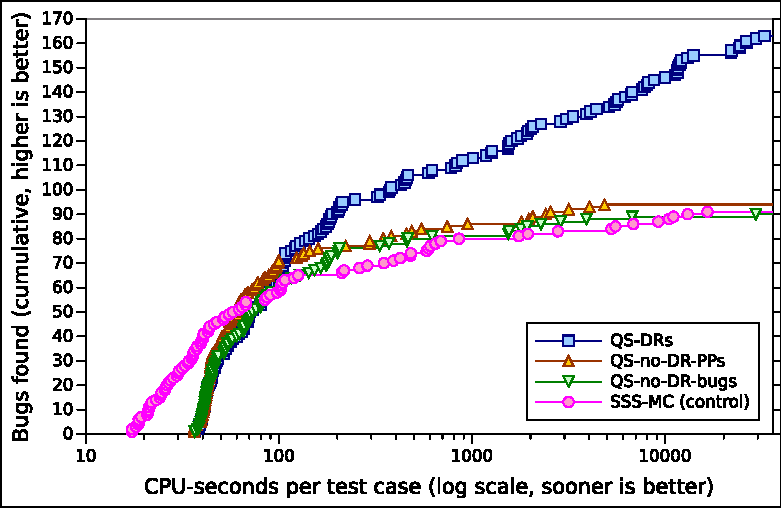
\includegraphics[width=0.48\textwidth]{dowefindbugsfaster-squashed.pdf} \\
		(a) Bugs found by elapsed CPU time. Overall, a more direct comparison than (b),
		although \quicksand's start-up overhead is exaggerated, as the SSS-MC tests are not parallelized. \\
		\\
	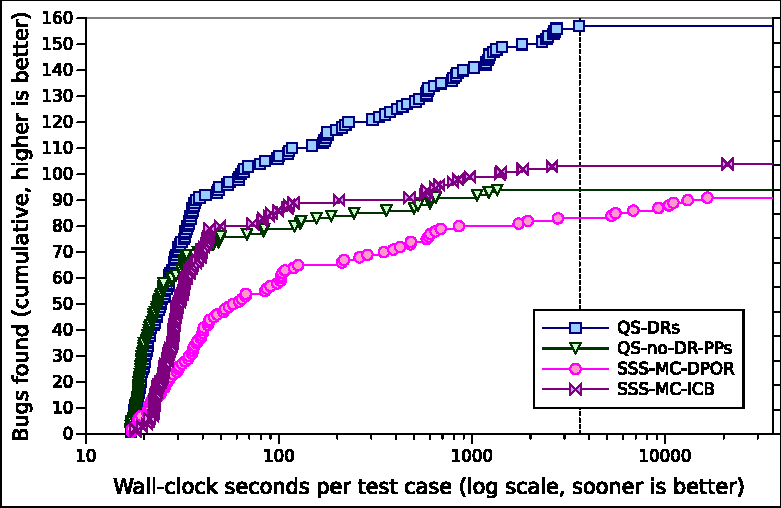
\includegraphics[width=0.48\textwidth]{dowefindbugsfaster-wallclock.pdf} \\
		(b) Bugs found by elapsed wall-clock time.
		\quicksand~is parallelized tenfold; the vertical line indicates its 1 hour limit. \\
	\end{tabular}
	}
	\caption{Comparison of bug-finding performance
	by several configurations of \quicksand~and the SSS-MC control.
	\quicksand~finds \revision{151}\% as many bugs with data-race PPs.}
	\label{fig:dowefindbugsfaster}
\end{figure}

{\bf Finding new data-race bugs.}
%We quickly pull ahead of SSS-MC, and ultimately conclude with 179\% as many bugs in total.
%The break-even point is at a negligible 90 seconds.
\revision{Compared to the best SSS-MC series, \quicksand~finds}~more bugs within any CPU budget greater than \revision{200}~seconds,
and ultimately concludes 10 CPU-hours with \revision{151}\% as many bugs in total.
\revision{Before the break-even point at 200 seconds,
% TODO
% (for SSS-MC-ICB) or XXX seconds (for SSS-MC-Shared-Mem)
\quicksand~lags behind the SSS-MC approaches due to additional start-up overhead from its tenfold parallelism.
However, converting SSS-MC's early CPU-time advantage into faster wall-clock performance remains an open research problem \cite{parallel-dpor}.
In Figure~\ref{fig:dowefindbugsfaster}(b), we give \quicksand~full credit for its inherent parallelism, and it outperforms SSS-MC for any fixed budget of wall-clock time.}

%{\bf Variance.}
% TODO CAMREADY: Probably will need at least a 3rd run of dis.
Because \quicksand~can be nondeterministic in its scheduling of state spaces,
we ran the QS-DR tests a second time to quantify the variance.
We found the area between the two QS-DR curves to be
% TODO
{\bf XX\%}
of the area between QS-DR and SSS-MC-ICB (the next closest),
% TODO cite
which we consider an insignificant amount of variance.
}


% TODO: Fix up this paragraph after preempt-everywhere results come in.
The left half of Table~\ref{tab:drbugs}
breaks down the number and types of bugs found by each test program.
In \mxtest, in which we do not trust the lock implementation's correctness,
the control experiment found dramatically fewer bugs (just 1)\footnote{
	The one bug SSS-MC found was in a fully-assembler lock implementation. {\tt yield()}'s return value clobbered a value stored in {\tt \%eax}, which could lead to a failure after two repeated contentions. Preempting only on {\tt yield()} (in the contention loop) was sufficient to find the bug.}.
%Intuitively, this is due to our control experiment being able to preempt only on the boundaries of the API which
%Though for many applications of MC, assuming a correct lock implementation is sufficient,
Though it often suffices to assume correctly-implemented locks,
we consider this strong evidence that new low-level synchronization code must be verified with data-race PPs.
%TODO CAMREADY: Run a mutex expt where "all atomic instrs" are PPs. See how many bugs are missed anyway.
% Wwe re-ran the \mxtest control experiment with \landslide~hard-coded to preempt on any atomic instruction
% (as well as on the mutex API boundaries).
% Still, this smarter configuration for SSS-MC found only 99999999999 bugs of \quicksand's 13.

%% RIP this.
%Furthermore, we plotted another line from this dataset, QS-no-DR-bugs,
%which represents only the bugs found in state spaces without any data-race PPs (like QS-no-DR-PPs, but paying any overhead for using data-race PPs).
%Intuitively, this line shows that for programs with only benign data races,
%\quicksand~can afford the extra overhead of verifying them while still slightly edging out SSS-MC.

% TODO: fix this table.
\begin{table*}[t]
	\begin{center}
		\small
	\begin{tabular}{r|c||c|c|c|c|c||c|c||c|c}
		% TODO: Update SSSMC column to have more favourable ICB numbers.
		& {\bf Num.} & {\bf DPOR} & {\bf QS} & {\bf DR-only} & {\bf Nondet.} & {\bf Malloc-} &
		{\bf Mutual} & {\bf Avg. tested} & {\bf Total} & {\bf Untested} \\
		{\bf Test name} & {\bf tested} & {\bf bugs} & {\bf bugs} & {\bf bugs} & {\bf DR bugs} & {\bf recycle DRs} &
		{\bf time-outs} & {\bf subset SSes} & {\bf DR PPs} & {\bf DR PPs} \\
		\hline
		% FIXME: update FRMs
				% #test  sssmc   qs      dronly  nondets  FRMs   timeout comp.SSes DRPPs untested DRPPs
		{\tt bcast}	& 79	& 7	& 11	& 4	& 4	& 51	& 0	& -	& 912	& 107	\\
		{\tt join} 	& 79	& 14 	& 24	& 10	& 6	& 333	& 5	& 60.8	& 781	& 292	\\
		{\tt mx} 	& 79	& 1	& 10	& 9	& 1	& 7	& 0	& -	& 829	& 1	\\
		{\tt sem} 	& 79	& 10	& 16	& 6	& 5	& 140	& 29	& 73.3	& 753	& 279	\\
		{\tt signal} 	& 79	& 4	& 10	& 7	& 6	& 180	& 10	& 54.2	& 1118	& 391	\\
		{\tt rwlock} 	& 79	& 26	& 28	& 2	& 2	& 125	& 19	& 29.6	& 915	& 634	\\
		\hline
		{\tt sched} 	& 59	& 1	& 7	& 6	& 4	& 0	& 0	& -	& 144	& 3	\\
		{\tt alarm} 	& 44	& 5	& 21	& 17	& 3	& 35 	& 22	& 9.1	& 115	& 89	\\
		{\tt wait} 	& 52	& 23	& 30	& 7	& 1	& 31	& 8	& 28.0	& 142	& 31	\\
		\hline
		{\bf Total}	& 629	& 91	& 157	& 68	& 32	& 902	& 93	& 42.6 	& 5709	& 1827	\\
	\end{tabular}
	\end{center}
	\caption{Summary of bugs and data races found by each test program.
		% TODO
		DPOR is the control; QS is \quicksand.
		``DR-only bugs'' counts among \quicksand's bugs how many required data-race PPs to expose (\sect{\ref{sec:eval-sssmc}});
	among those, ``Nondeterministic DR bugs'' counts how many candidates required MC integration to identify (\sect{\ref{sec:eval-dr}}).
	``Malloc-recycle DRs'' counts how many false positives we suppressed (\sect{\ref{sec:eval-dr}}).
	``Mutual time-outs'' counts how often both SSS-MC and \quicksand~timed out with no bug found;
	among those, ``Average tested subset SSes'' counts how many partial verifications \quicksand~provided on average for each test (\sect{\ref{sec:eval-sssmc}}).
	``Total DR PPs'' counts how many unique data-racing instructions we identified among tests where we found no bugs;
	among those, ``Untested DR PPs'' counts how many could not be checked in the time limit (\sect{\ref{sec:future}}).
		}
	\label{tab:drbugs}
\end{table*}

% TODO CAMREADY: Compare QS-ETAs to QS-Random to evaluate "smaller is better" claim.
{\bf Finding the same bugs faster.}
%To test whether Iterative Deepening is effective even for MC domains without data races, %such as message-passing distributed systems,
\revision{The QS-Sync-Only experiment tests whether}~Iterative Deepening is effective even for MC domains without data races.
\revision{When \quicksand~ignores all data-race candidates,
its results are competitive with SSS-MC-DPOR, but SSS-MC-ICB outperforms it.
This is unsurprising: the seed subsets of PPs (\sect{\ref{sec:initial-pp}}) QS-Sync-Only is limited to are much less flexible than ICB's preemption strategy.
This result suggests that in future work, \quicksand~should consider using ICB in parallel with its default configuration when it finds no data-race candidates to test.}
%\footnote{
%Because \quicksand~is not yet instrumented to subset hard-coded PPs beyond the 4 ways shown in Figure~\ref{fig:id},
%we ran these tests for 2.5 hours on 4 CPUs each.
%Future work could parallelize QS-no-DR-PPs further; see \sect{\ref{sec:future}}.}.

%Even though SSS-MC mostly catches up to it by the end of the 10-hour budget,
%and is faster in the first 60 seconds due to less start-up overhead,
%QS-no-DR-PPs finds more of the bugs sooner thereafter.
%Hence, for modest CPU budgets,
%\quicksand~is likely to find bugs SSS-MC will miss.
%and for more ambitiously-sized tests,
%programmers can be more confident in the verification provided when \quicksand~times out with no bug found.
%We conclude that for smaller arbitrary CPU budgets, especially less than 1 hour,
%Iterative Deepening is likely to find bugs SSS-MC will miss.
%Moreover, it is also easy to imagine scaling up the size of each test case to test ,
%using more threads or longer sequences of API calls.
%We hope that is compelling even to users willing to spend many CPU-hours on testing.
%These results show explicitly that for arbitrary CPU-time budgets
%\footnote{The initial perfect overlap between QS-DRs and QS-no-DR-bugs indicates how long it takes before the first data-race bug is found.}
%even after the extra overhead of verifying them, \quicksand~still slightly edges out SSS-MC

\revision{
On the other hand,
comparing QS-DR to SSS-MC-Shared-Mem shows that Iterative Deepening thoroughly outperforms ICB when shared-memory preemptions come into play.
%We attribute this to the fact that
Statically configuring a PP for every shared memory access in advance
produces orders of magnitude more PPs than
waiting for an access to be identified as part of a (potential) data race at runtime.
%
In principle, DPOR and BPOR should identify and prune any equivalences arising from extraneous PPs on non-conflicting accesses.
However, in practice,
%we found that
the sheer number of accesses during each new execution (often thousands) added significant performance overhead to the MC when computing DPOR and backtracking\footnote{
	\revision{The bug-finding performance of SSS-MC-ICB approach could be improved by heuristically
	%preempting only on data-race candidates found in advance by a single-pass analysis
	using a single-pass analysis to find data-race PP candidates in advance
	\cite{portend}, but this sacrifices soundness, as shown in \sect{\ref{sec:eval-dr}}.}
}.
Iterative Deepening avoids this overhead by waiting until runtime to identify fewer, more relevant PPs dynamically,
and is hence more suitable for MC with data-race PPs.}

{\bf Partial verification.}
When a MC job times out, the user may prefer a brief summary of what parts of the test were verified, rather than writing off all the CPU time as a waste.
%Beyond using the state space estimator to guess the percent coverage,
We know of no approach to quantify the probability
that a bug would be exposed by an untested interleaving,
but \quicksand~at least reports which subsets of PPs resulted in state spaces that did complete in time.
%\quicksand~does not attempt any such quantitative guarantee,
%but can at least report
On 129 tests, the SSS-MC control experiment timed out after 10 hours with no bugs found.
Among these tests, \quicksand~found bugs in 36.
For the other 93, we show the number of state spaces \quicksand~was able to complete in the ``Average tested subset SSes'' column of Table~\ref{tab:drbugs}.
%and the number of unique PPs among them.
%In 6 cases, \quicksand~also failed to complete anything; beyond these,
%between 1 and 253 state spaces were completed for each test
%Between 0 and 233 unique PPs were tested among some completed subsets, with a mean of 27.2 and median of 7.5.
These completions guarantee that, if the test program could expose a bug,
% Justify implicit hypothesis: Sync PPs + DR PPs = all possible relevant PPs.
it would only be found by a new data-race PP not discovered yet, or by a superset combination of PPs not reached.

%Hence, in Table~\ref{tab:drbugs} we count how often \quicksand~uncovered a bug only in state spaces which included data-race PPs, while
%
%In Table~\ref{tab:allbugs} ....

{\bf Full verification.}
% TODO: Discuss how ICB sucks even more.
For 153 of our 629 tests, \quicksand~was able to provide the total verification guarantee described in \sect{\ref{sec:totalverif}}.
In Figure~\ref{fig:totalverif} we plot the cumulative distribution of \quicksand's total verifications
%before a given elapsed CPU consumption.
\revision{against those provided by SSS-MC-Shared-Mem\footnote{
	\revision{In kernel or thread library code, a thread's own stack accesses may not always be private. %assumption may not hold.
	For example, many P2 condvars use stack-allocated list nodes to track waiting threads.
	SSS-MC-Shared-Mem's verifications are only sound in the absence of such sharing!
	\quicksand~detects these dynamically, without needing to discriminate between stack and heap.}
	%Expanding the statically-coded PPs to include stack accesses would make SSS-MC-Shared-Mem's performance even worse.
	% Especially for testing kernel-level code, deciding which of a thread's memory accesses are shared versus private is nonstraightforward, as threads may share data structures allocated on their own stacks for synchronization. Hence, the common heuristic of ignoring stack accesses as private (which we employ for this control experiment) introduces some unsoundndess.
}.
\quicksand~outperforms SSS-MC, being able to verify safety for
% TODO
{\bf 99x}
as many tests in 10 CPU-hours.
We attribute this again to the overhead of the sheer number of statically-coded PPs that SSS-MC-Shared-Mem must use,
as well as to the work which ICB necessarily repeats when increasing its preemption bound.}

Among these verified tests, 36 contained no data-race candidates whatsoever,
so the same verification could be provided
%by SSS-MC
\revision{with synchronization PPs only.
We plot the verifications by QS-Sync-Only, SSS-MC-DPOR and SSS-MC-ICB as well:
among these, the otherwise more antiquated SSS-MC-DPOR performs best,
while the other two lag behind
}
%\quicksand~is slower than SSS-MC-DPOR
due to redundant work (\sect{\ref{sec:future}}).
\revision{While QS-Sync-Only and SSS-MC-ICB are competitive with each other},
using data-race PPs increases our \revision{verification capacity}~by 4.25x.

\begin{figure}[t]
	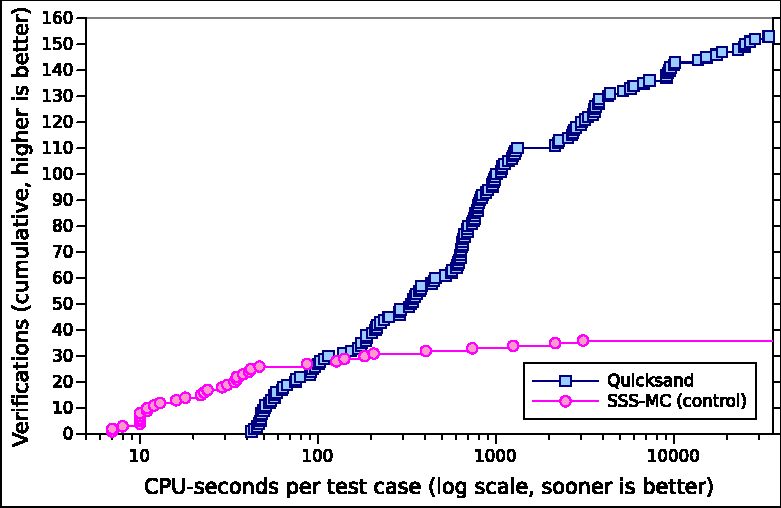
\includegraphics[width=0.48\textwidth]{totalverifs-squashed.pdf}
	\caption{Cumulative distribution of tests \quicksand~fully verified (\sect{\ref{sec:totalverif}}).
	Some tests had no data-race candidates, and hence could also be verified by SSS-MC.}
	\label{fig:totalverif}
\end{figure}


%%%%%%%%%%%%%%%%%%%%%%%%%%%%%%%%%%%%%%%%%%%%%%%%%%%%%%%%%%%%%%%%%%%%%%%%%%%%%%%%

\subsection{Comparing to single-pass data-race analysis}
\label{sec:eval-dr}
% Though we mechanically verify whether each data race candidate leads to a bug, each new PP can increase combinatorially..... obviously wish to avoid...

Beyond finding new bugs with data-race PPs, we evaluated \quicksand's performance for classifying data-race candidates in two ways.

{\bf Suppressing ``malloc-recycle'' false positives.}
In \sect{\ref{sec:recycle}} we showed the soundness of suppressing data race reports between two heap accesses when the surrounding memory was re-allocated in between.
In Table~\ref{tab:drbugs}, the column ``Malloc-recycle DRs'' shows the total number of such data-race candidates for each test program.
In total, 902 data-races fit the malloc-recycle pattern across all tests,
only 69 of which were observed to avoid the re-allocation in an alternate interleaving.
Our proof in \sect{\ref{sec:recycle}} guarantees the safety of pruning all 833 other state spaces.

Among those 69 true data-races, %which initially fit the malloc-recycle pattern,
none exposed a new bug when used as a PP.
This suggests that for other data-race tools,
suppressing malloc-recycle candidates may be a productive heuristic,
even if unsound without Iterative Deepening.
However, \quicksand~was able to correctly identify the 69 violations of that heuristic (among 30 distinct tests),
and fall back to classifying them with DPOR.
%which we consider a much stronger verification.

%%%%%%%%%%%%%%%%%%%%%%%%%%%%%%%%%%%%%%%%%%%%%%%%%%%%%%%%%%%%%%%%%%%%%%%%%%%%%%%%

%For the [NONDET] expt, you don't need to additionally count how many DRs
%needed to be found in a DR-PP state space, because when EXPLORE_BACKWARDS=0,
%you'll need to preempt on the DR PP to find the new DR anyway, hence they will
%be nondet. Unless you want to separately count the subset of nondet drs that
%are also dr-pp-ss-only (the reviewers may ask for this before cam-ready?).
{\bf \revision{Finding nondeterministic data-race candidates}.}
Some memory accesses may be hidden in a control flow path that requires a nondeterministic preemption to be executed.
In such cases, a single-pass dynamic data-race detector
%could not achieve the coverage necessary
could fail
to identify a racing access pair as a candidate to begin with.
%
We counted how many such data-races, used as PPs, led to \quicksand~finding new bugs,
thereby making them {\em false negatives} of the single-pass approach.
We classified each data-race candidate according to whether \landslide~reported them during the first interleaving,
before any backtracking or preempting:
if so, they were {\em single-pass data races}; otherwise, {\em nondeterministic}.

To ensure a fair comparison, we disabled \landslide's {\em false-positive}-avoidance techniques during this experiment.
For example, we reported malloc-recycle data races during the first interleaving, as a single-pass analysis must
%rather than waiting until future interleavings to witness them without the malloc-recycle pattern
(\sect{\ref{sec:recycle}}).
This prevents \landslide~from suppressing an observed data race on the first interleaving,
which would falsely classify it as nondeterministic.

\begin{figure}[t]
	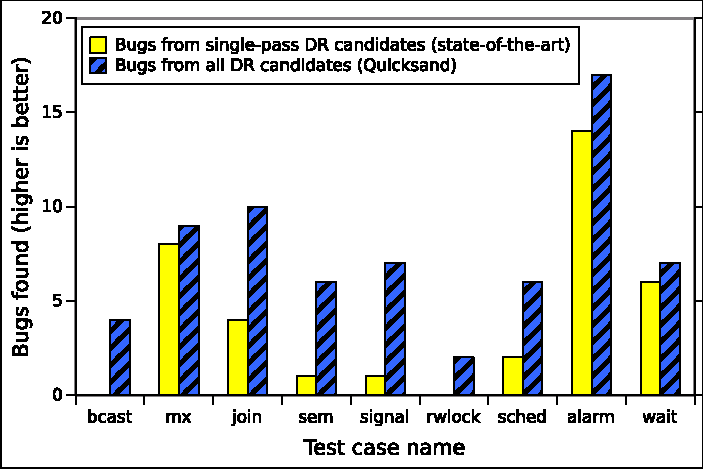
\includegraphics[width=0.48\textwidth]{nondet-drs-1-v2.pdf}
	\caption{Some data-race candidates may not be identified during a single program execution.
		Using nondeterministic data races as PPs,
		\quicksand~found 189\% as many data-race bugs compared to using single-pass candidates alone.
	}
	\label{fig:dr-falsenegs}
\end{figure}
Figure~\ref{fig:dr-falsenegs} compares the types of data-race candidates necessary to expose each data-race bug in our test suite.
The first series represents the bugs found using PPs from single-pass data-race candidates,
% not entirely true, as portend could be given data-race traces from an MC,
%but they don't do it in their paper, so i feel comfortable making this claim
i.e., the state-of-the-art approach used by \cite{racefuzzer,portend}.
The second series shows all data-race bugs \quicksand~found,
which includes the former type as well as new bugs involving nondeterministic data-races.
\quicksand~found 68 data-race bugs in total, only 36 of which could be found with single-pass data-race candidates alone.
%In total, we found 189\% as many bugs by using nondeterministic data-race candidates as PPs.

%When proving that [NONDET] dr buges exist, make sure to mention that, although
%their frequency varies depending on test case (mx test: almost none; bct:
%almost all), they are still PRESENT in all (or almost all) test cases, meaning
%it is not just a matter of writing better test cases.

Note that we are not comparing how much testing time is required before identifying the data-race candidates involved in each bug.
Single-pass data races can all be found after a single program execution,
while \quicksand~may potentially take up to all 10 CPU-hours before identifying a nondeterministic data race.
However, prior work data-race tools \cite{tsan}, being not integrated with a MC,
are not intended to discover new candidates under subsequent runs.
Running a single-pass data-race tool repeatedly for 10 CPU-hours could potentially uncover some nondeterministic candidates,
but stress testing's comparative problem with achieving reliable coverage is already well-understood
\cite{chess-icb,gambit}.
Likewise, replay-based tools \cite{portend} are dependent upon the data-race detector to provide an execution trace leading to each candidate.
This experiment suggests that
such tools could benefit from a similar feedback loop as used in Iterative Deepening.
%i.e., discovering transitively-reachable data races while testing initial ones.
%although that would still not simultaneously be able to provide total verifications.
% TODO: read gambit paper


% Figure out concretely what the data race tricks are that we do, so we can claim them as contributions in the paper. Then ACTUALLY EVALUATE THEM.
%         - Speculative DR PPs.
%                 Not a heuristic, rather how to make it work at all to begin with.
%                 (Cite MS thesis, claim on backwards explorating finding bugs faster)
%         - Free/re-malloc to eliminate some false positives. See #193.
%                 Measure how many false positives are eliminated.
%                 Check, ofc, to make ABSOLUTE SURE, that no bugs missed w/ this trick.
%                         If there are, it could be because of the implementation
%                         bug described in #193.
%         - Using tid/last_call filtering because whole stack traces are too expensive.
%                 Moderately optional, 1st priority since theoretically interesting:
%                 Turn on/off and measure how resulting DR bug #s change.
%         - Optional: Reprioritizing DRs based on "confirmed" / "suspected"
%                 Shouldn't be hard just make ID wrapper print "s" or "c"!
%                 Is it helpful for ID to put priorities on DR PPs?
%                         Test by inverting the priority and see if fewer buges are found.
%         // Super optional to talk about. Probably not worth the time.
%         // - "Too suspicious" (during init/destroy)
%         //      (Cite eraser, section 2.2)

\section{Related Work}
\label{sec:related}

\subsection{Stateless Model Checking}

We build upon many established model-checking techniques, dating back
% of course
to Verisoft, the original C model checker \cite{verisoft}.
%, and Eraser, the original data race detector \cite{eraser}.
%Our model checker
%\landslide~\cite{landslide} itself implements many techniques from prior work (\sect{\ref{sec:landslide}}).
%itself implements DPOR \cite{dpor},
%state space estimation \cite{estimation},
%and data-race detection \cite{eraser}.
We compare related tools by their treatment of shared-memory thread communication.

{\bf Synchronization events only.} CHESS \cite{chess} and dBug \cite{dbug-ssv} instrument the thread library API, and can preempt programs only during calls to this API.
Hence, they will miss any bugs that require interleaving threads at instruction granularity during a data race. CHESS provides a data-race analysis to report any such violations of its concurrency model to the user, but does not incorporate data-race candidates as PPs in future tests.

{\bf Message-passing.} Other stateless model checkers, such as SAMC \cite{samc}, MaceMC \cite{macemc}, MoDist \cite{modist}, ETA \cite{dbug-retreat}, and Concuerror \cite{optimal-dpor},
limit thread communication to a message-passing API to more effectively test distributed systems.
This eliminates the need for data-race analysis, but restricts the class of programs that can be tested.
Nevertheless, Iterative Deepening is applicable to these tools.

{\bf Preempting at instruction granularity} is a prerequisite for using data-race PPs.
However, the resulting state space explosion demands that any such tool either
choose a small subset of instructions to consider as PPs
or be limited to very small test programs.
%However, every such prior tool we know of has serious drawbacks.
SKI \cite{ski} approaches kernel code by statically choosing a random set of instructions in advance, %offsets from the start of the test,
which is perhaps more similar to
%stress testing or
schedule fuzzing \cite{randomized-scheduler} than to exhaustive state space exploration.
%
SPIN \cite{spin} specializes in verifying synchronization primitive implementations such as RCU \cite{rcu}, which is similar to our \mxtest~experiment,
although it requires code to be written in the PROMELA language.
%However, SPIN is stateful rather than stateless, and explicitly storing visited program states rather than using DPOR limits the size of programs that can be practically tested.
%
Inspect \cite{inspect} instruments source code by inserting wrapper calls around all accesses to potentially-shared data.
It identifies such instructions in advance with an over-approximating alias analysis,
while \landslide~\cite{landslide} traces the memory locations of accesses at runtime.
Both SPIN and Inspect fix their set of PPs in advance, so could be
%combined with \quicksand~
extended with Iterative Deepening in future work.
%so cannot check implementations directly.

{\bf Other techniques.} Various improvements or alternatives to DPOR have been developed, such as Dynamic Interface Reduction \cite{demeter}, Maximal Causality Reduction \cite{mcr},
%DPOR for relaxed memory models \cite{tsopso},
and SAT-directed MC \cite{satcheck}.
These are all compatible with our technique.
Recent work \cite{tsopso} has extended DPOR for relaxed memory models \cite{memory-consistency-models},
which we do not yet account for in our proofs (\sect{\ref{sec:soundness}}).
Parrot \cite{parrot} combines MC with a partially-determinizing runtime for further reduction, but still, fewer than half the non-trivial state spaces in their evaluation could be completed.
%providing a strong argument for \quicksand.
Finally, Iterative Context Bounding (ICB) \cite{chess-icb} is most similar to our work,
as both approaches provide a partial verification
%on some subset of interleavings
when full completion is intractable (\sect{\ref{sec:future}}).
However, ICB is limited to a fixed set of PPs, and to our knowledge no algorithm has been proposed to dynamically add data-race PPs during a test with ICB.

\subsection{Data Race Detection}
\label{sec:related-dr}

%Too many related projects to list have made contributions to the
Many advances have been made on the false-positive data race problem since it was first introduced in \cite{eraser}.
\cite{hybriddatarace} and \cite{tsan} combine the lockset and happens-before analyses into a hybrid technique, which we employ.
DroidRacer \cite{droidracer} and CAFA \cite{cafa} target
%event-driven
Android applications, using domain-specific heuristics (orthogonal to our method) to reduce false positives. % cut for space?
Like \landslide, DataCollider \cite{datacollider} offers data-race techniques for kernel code.
IFRit \cite{ifrit}
improves performance using an interference analysis,
which would allow future work to avoid tracing every memory access.
%although in our context, we cannot admit false negatives (\sect{\ref{sec:totalverif}}).
% No, IDGAF about pure happens before.
%FastTrack \cite{fasttrack} optimizes the performance of pure happens-

Closer to our work, replay analysis \cite{recordreplaydrs} also suppresses false positives by testing multiple thread interleavings.
%after finding data race candidates.
This work compares the immediately resulting program states for differences,
preferring to err on the side of false positives.
RaceFuzzer \cite{racefuzzer} avoids false positives by requiring an actual failure be exhibited, as we do,
although it uses random schedule fuzzing rather than stateless MC.
While this technique can also classify malloc-recycle candidates as false positives (\sect{\ref{sec:recycle}}),
they require replaying the threads in a new interleaving.
Moreover, \cite{portend} argues that accurate classification may require many re-executions,
%according to many pre- and post-race sequences,
which is tantamount to adding a new state space in \quicksand.
Our proof in \sect{\ref{sec:recycle}} allows us to eliminate this special case with no additional replay beyond what DPOR already requires.

Portend \cite{portend} is the most closely related work we have found.
Based on single-pass data race reports, it tests alternate program executions to classify candidates in a taxonomy of likely severity.
It uses symbolic execution to test input nondeterminism as well as schedule nondeterminism,
%while we explore the latter only.
and additionally reports non-failing races which nevertheless cause
%suspiciously
different program output. %, which is orthogonal to our technique.
However, Portend does not test alternate interleavings {\em in advance} of knowing any specific data races,
which is necessary to expose certain bugs (\sect{\ref{sec:eval-falseneg}}) or to provide full verification (\sect{\ref{sec:totalverif}}).
% Not really true.
%It also assumes the POSIX synchronization API, so cannot verify arbitrary synchronization algorithms such as we do with \mxtest.
Future work could combine the two approaches, using MC to produce new data-race traces for Portend to classify, or using Portend's analysis to inform \quicksand's heuristic priorities.

% \subsection{Other Concurrency Testing Approaches}
%
% blah blah pldi'15 symbiosis DSP

% Note that BPOR paper claims that ICB(3+) repeats LOADS of work, and that makes it ok for landslide-ID to repeat work.

% IDK if i should mention it, but OOPSLA 2015, protocol based verification of MPI concurrency paper. Different verification approach entirely; doesn't suffer exponential explosion but limited to programs with no shared state and MPI communication only

% Probably NOT worth a mention: OOPSLA 2015, stateless model checking of event driven applications. Turning timer-driven model on its head and checking single-threaded, but asynch-event-driven programs (i.e. device-like signal handlers)


%%%%%%%%%%%%%%%%%%%%%%%%%%%%%%%%%%%%%%%%%%%%%%%%%%%%%%%%%%%%%%%%%%%%%%%%%%%%%%%%

\section{Conclusion}

%We are great. Accept our paper.

We have presented \quicksand, an implementation of Iterative Deepening, a new technique for automating the choice of PPs during stateless model checking.
% , and \quicksand, a tool which implements this technique tailored to the \landslide~model checker.
\quicksand~incorporates \landslide's data-race analysis to create new PPs tailored specifically to the program under test,
and manages multiple \landslide~instances to test many different PP subsets in a given CPU budget, even when the full state space of all PPs would be computationally intractable.

Our evaluation shows that \quicksand~achieves better bug-finding results than either single-pass data-race detection or single-state-space model checking (SSS-MC) alone.
We dramatically reduce false-positive data race reports,
%by verifying the absence of bugs in their associated state spaces
and find crashes caused by nondeterministic data-races in alternate thread interleavings missed entirely by single-pass analysis.
Compared to SSS-MC, we find bugs faster in smaller subset state spaces,
%when the maximal state space is too large to explore
and find new bugs with data-race PPs that the maximal state space would not expose at all.

Although \landslide~itself is not publicly available due to its dependency on the non-free simulator \simics, \quicksand~is open-source and its interface can be adapted to fit any similar tool.
We have also posted the log files from all our experiments.
They can be found here:

\url{https://github.com/bblum/landslide} % TODO: put QS in its own repository

\url{https://github.com/bblum/landslide} % TODO: put final logs somewhere

\section{Acknowledgements}

Many thanks to David A. Eckhardt, Vaishaal Shankar, and Haryadi Gunawi for generously providing student implementations from CMU's, Berkeley's, and U. of Chicago's OS classes respectively.
Thanks to Wind River for the use of their simulator \simics, upon which \landslide~is built.
Thanks to Ji\v{r}\'{i} \v{S}im\v{s}a and the anonymous PLDI reviewers for their helpful comments.
This work was supported in part by % TODO: funding sources


\bibliographystyle{abbrvnat}
\bibliography{citations}{}

\end{document}
